\section{Motivação}
\label{motivacao}

O novo coronavírus, chamado síndrome respiratória aguda grave coronavírus 2 (SARS-CoV-2), que causa a doença COVID-19 \cite{sars-name}, foi declarado uma pandemia pela Organização Mundial de Saúde (WHO) em março de 2020 \cite{oms}. O vírus causou sintomas em mais de 260 milhões de pessoas ao redor do mundo, trazendo mais de 5 milhões de mortes ao total, até novembro de 2021 \cite{contagem-global}.

No Brasil, o terceiro país mais afetado mundialmente, houveram mais de 22 milhões de casos registrados, com cerca de 610 mil mortes registradas \cite{contagem-global}. Enquanto em Recife, Pernambuco, até setembro de 2021, 610 mil casos foram documentados pela Prefeitura do Recife \cite{casosleves}, com 30 mil sendo classificados como casos graves, e cerca de 7 mil destes resultando no óbito do paciente \cite{casosgraves}. A vacinação é uma das medidas que a Organização Mundial de Saúde (OMS) propõe para a prevenção da doença, e está em progresso no Recife desde janeiro de 2021 \cite{vacinometro}. É estimado que até setembro de 2021, cerca de 65\% da população \cite{populacaorecife} tivesse a dosagem recomendada da vacina, com duas doses ou doses únicas.

Embora os sintomas da doença sejam tosse seca, falta de ar, febre, dor de cabeça, dor de garganta e fadiga, uma parte indefinida dos casos é assintomática, ou seja, não apresentam sintomas, mas ainda carregam e espalham o vírus. Certos casos da doença podem evoluir em gravidade, similar a um caso de pneumonia grave, podendo causar morte. Percebe-se que casos mais graves da doença geralmente ocorrem em pessoas idosas ou com doenças crônicas, como diabetes, hipertensão arterial, doenças cardíacas e respiratórias \cite{patologia}.

Neste contexto de ampla coleta de dados pela Prefeitura do Recife, é possível então aplicar modelos de aprendizagem de máquina com o intuito de compreender e prever a doença e sua possível evolução em certos pacientes. Esta abordagem se provou eficaz em diversos estudos nacionais e internacionais, discutidos na seção \ref{sec:trabalhos}. Porém, não foram identificados estudos focados na população da cidade do Recife ou que apliquem aprendizagem de máquina considerando o progresso da vacinação em uma região específica como atributo.


% \begin{figure}[ht!]
\centering

\caption{\textmd{Introdução 1}}
\label{fig:figuraex}
\fcolorbox{gray}{white}{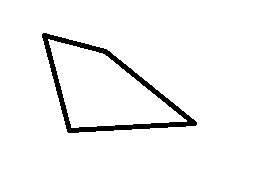
\includegraphics[width=0.5\textwidth]{chapters/introducao/images/figuraex.png}}

\par\medskip\ABNTEXfontereduzida\selectfont\textbf{Fonte:} \citeauthor{manualufpe2020} (\citeyear{manualufpe2020}) \par\medskip
\end{figure}
